% Preámbulo
\documentclass[letterpaper]{article}
\usepackage[utf8]{inputenc}
\usepackage[spanish]{babel}

\usepackage{enumitem}
\usepackage{titling}

% Símbolos
	\usepackage{amsmath}
	\usepackage{amssymb}
	\usepackage{amsthm}
	\usepackage{amsfonts}
	\usepackage{mathtools}
	\usepackage{bbm}
	\usepackage[thinc]{esdiff}
	\allowdisplaybreaks

% Márgenes
	\usepackage
	[
		margin = 1.2in
	]
	{geometry}

% Imágenes
	\usepackage{float}
	\usepackage{graphicx}
	\graphicspath{{imagenes/}}
	\usepackage{subcaption}

% Ambientes
	\usepackage{amsthm}

	\theoremstyle{definition}
	\newtheorem{ejercicio}{Ejercicio}

	\newtheoremstyle{lemathm}{4pt}{0pt}{\itshape}{0pt}{\bfseries}{ --}{ }{\thmname{#1}\thmnumber{ #2}\thmnote{ (#3)}}
	\theoremstyle{lemathm}
	\newtheorem{lema}{Lema}

	\newtheoremstyle{lemathm}{4pt}{0pt}{\itshape}{0pt}{\bfseries}{ --}{ }{\thmname{#1}\thmnumber{ #2}\thmnote{ (#3)}}
	\theoremstyle{lemathm}
	\newtheorem{sol}{Solución}
	
	\newtheoremstyle{lemathm}{4pt}{0pt}{\itshape}{0pt}{\bfseries}{ --}{ }{\thmname{#1}\thmnumber{ #2}\thmnote{ (#3)}}
	\theoremstyle{lemathm}
	\newtheorem{theo}{Teorema}

	\newtheoremstyle{lemademthm}{0pt}{10pt}{\itshape}{ }{\mdseries}{ --}{ }{\thmname{#1}\thmnumber{ #2}\thmnote{ (#3)}}
	\theoremstyle{lemademthm}
	\newtheorem*{lemadem}{Demostración}

% Macros
	\newcommand{\sumi}[2]{\sum_{i=#1}^{#2}}
	\newcommand{\dint}[2]{\displaystyle\int_{#1}^{#2}}
	\newcommand{\inte}[2]{\int_{#1}^{#2}}
	\newcommand{\dlim}{\displaystyle\lim}
	\newcommand{\limxinf}{\lim_{x\to\infty}}
	\newcommand{\limninf}{\lim_{n\to\infty}}
	\newcommand{\dlimninf}{\displaystyle\lim_{n\to\infty}}
	\newcommand{\limh}{\lim_{h\to0}}
	\newcommand{\ddx}{\dfrac{d}{dx}}
	\newcommand{\txty}{\text{ y }}
	\newcommand{\txto}{\text{ o }}
	\newcommand{\Txty}{\quad\text{y}\quad}
	\newcommand{\Txto}{\quad\text{o}\quad}
	\newcommand{\si}{\text{si}\quad}

	\newcommand{\etiqueta}{\stepcounter{equation}\tag{\theequation}}
	\newcommand{\tq}{:}
	\renewcommand{\o}{\circ}
	\newcommand*{\QES}{\hfill\ensuremath{\blacksquare}}
	\newcommand*{\qes}{\hfill\ensuremath{\square}}
	\newcommand*{\QESHERE}{\tag*{$\blacksquare$}}
	\newcommand*{\qeshere}{\tag*{$\square$}}
	\newcommand*{\QED}{\hfill\ensuremath{\blacksquare}}
	\newcommand*{\QEDHERE}{\tag*{$\blacksquare$}}
	\newcommand*{\qel}{\hfill\ensuremath{\boxdot}}
	\newcommand*{\qelhere}{\tag*{$\boxdot$}}
	\renewcommand*{\qedhere}{\tag*{$\square$}}

	\newcommand{\suc}[1]{\left(#1_n\right)_{n\in\N}}
	\newcommand{\en}[2]{\binom{#1}{#2}}
	\newcommand{\upsum}[2]{U(#1,#2)}
	\newcommand{\lowsum}[2]{L(#1,#2)}
	\newcommand{\abs}[1]{\left| #1 \right| }
	\newcommand{\bars}[1]{\left \| #1 \right \| }
	\newcommand{\pars}[1]{\left( #1 \right) }
	\newcommand{\bracs}[1]{\left[ #1 \right] }
	\newcommand{\inprod}[1]{\left\langle #1 \right\rangle }
    \newcommand{\norm}[1]{\left\lVert#1\right\rVert}
	\newcommand{\floor}[1]{\left \lfloor #1 \right\rfloor }
	\newcommand{\ceil}[1]{\left \lceil #1 \right\rceil }
	\newcommand{\angles}[1]{\left \langle #1 \right\rangle }
	\newcommand{\set}[1]{\left \{ #1 \right\} }
	\newcommand{\norma}[2]{\left\| #1 \right\|_{#2} }


	\newcommand{\NN}{\mathbb{N}}
	\newcommand{\QQ}{\mathbb{Q}}
	\newcommand{\RR}{\mathbb{R}}
	\newcommand{\ZZ}{\mathbb{Z}}
	\newcommand{\PP}{\mathbb{P}}
    \newcommand{\EE}{\mathbb{E}}
	\newcommand{\1}{\mathbbm{1}}
	\newcommand{\eps}{\varepsilon}
	\newcommand{\ttF}{\mathtt{F}}
	\newcommand{\bfF}{\mathbf{F}}

	\newcommand{\To}{\longrightarrow}
	\newcommand{\mTo}{\longmapsto}
	\newcommand{\ssi}{\Longleftrightarrow}
	\newcommand{\sii}{\Leftrightarrow}
	\newcommand{\then}{\Rightarrow}

	\newcommand{\pTFC}{{\itshape 1er TFC\/}}
	\newcommand{\sTFC}{{\itshape 2do TFC\/}}


% Datos
    \title{Métodos Estadísticos \\ Tarea 1}
    \author{Rubén Pérez Palacios Lic. Computación Matemática\\Profesor: Dr. Rogelio Ramos Quiroga}
    \date{\today}

% DOCUMENTO
\begin{document}
	\maketitle
	En un estudio se examina hojas de plantas y se cuenta el número de cierto tipo de insectos. Suponga que la distribución del número de insectos por hoja es una Poisson con media $\lambda$. Ahora, en muchas hojas no hay insectos pues no son adecuadas como alimento para los insectos, de aquí que se decide no considerar hojas en donde no haya insectos.
	\begin{enumerate}
		\item Obtenga la probabilidad de que en una hoja haya $i$ insectos, dado que hay al menos uno.
		
		\begin{sol}
			Sea $X\sim Poisson\pars{\lambda}$. Por definición de probabilidad condicional tenemos que

			\[\PP\bracs{X = i| X > 0} = \frac{\PP\bracs{X = i, X > 0}}{\PP\bracs{X > 0}}.\]

			Consideremos 2 casos. Cuando $i = 0$ entonces $\PP\bracs{X = i, X > 0} = 0$ por lo que 

			\[\PP\bracs{X = i| X > 0} = 0,\]

			en cambio cuando $i > 0$ entonces $\set{X = i} \subset \set{X > 0}$, por lo que $\PP\bracs{X = i, X > 0} = \PP\bracs{X = i}$ y por lo tanto

			\[\PP\bracs{X = i| X > 0} = \frac{\PP\bracs{X = i}}{\PP\bracs{X > 0}} = \frac{\PP\bracs{X = i}}{1-\PP\bracs{X = 0}} = \frac{\lambda^{i}e^{-\lambda}}{i! \pars{1-e^{-\lambda}}}.\]


		\end{sol}
		\item Suponga que se observan $x_1$ hojas con $1$ insecto, $x_2$ hojas con $2$ insectos, etc., donde $\sum_{i} x_{i} = n$. Muestre que el estimador de máxima verosimilitud, $\hat{\lambda}$, del parámetro $\lambda$, satisface la ecuación
		\[\hat{\lambda} = \tilde{x}\pars{1-e^{-\hat{\lambda}}}\]
		donde $\tilde{x} = \sum_{i} ix_i/n$.

		\begin{proof}
			Primero puesto que $\sum_{i} x_{i} = n$ entonces la cantidad de hojas con insectos son $n$, enumeramos estas hojas del $1-n$ y representando por $y_{i}$ la cantidad de insectos en la hoja $i$. La cantidad de insectos entre todas las hojas es por definición $\sum_{i} ix_{i} = \sum y_{i}$.

			De ahora en adelante trabajaremos con la muestra $y_{i}$. La función de verosimilitud esta dada por

			\[L\pars{\lambda} = \prod_{i=1}^n \PP\bracs{Y_{i} = y_{i}} = \prod_{i=1}^n \frac{\lambda^{y_{i}}e^{-\lambda}}{y_{i}! \pars{1-e^{-\lambda}}} = \pars{\frac{\pars{\lambda^{\overline{y}}}e^{-\lambda }}{\pars{1-e^{-\lambda}}}}^n \prod_{i=1}^n \frac{1}{y_{i}!},\]

			por lo que la logverosimilitud haciendo uso de propiedades del logaritmo es

			\[l\pars{\lambda} = \log\pars{\pars{\frac{\pars{\lambda^{\overline{y}}}e^{-\lambda }}{\pars{1-e^{-\lambda}}}}^n \prod_{i=1}^n \frac{1}{y_{i}!}} = n\overline{y}\log\pars{\lambda} - n\lambda - n\log\pars{1-e^{-\lambda}} + \sum_{i=1}^n\log\pars{\frac{1}{y_{i}!}}\]

			con $\overline{y} = \sum_{i} y_i/n$, de donde obtenemos la función score haciendo uso de propiedades de la derivada es

			\[S\pars{\lambda} = \diff{n\overline{y}\log\pars{\lambda} - n\lambda - n\log\pars{1-e^{-\lambda}} + \sum_{i=1}^n\log\pars{\frac{1}{y_{i}!}}}{\lambda} = \frac{n\overline{y}}{\lambda} - n - \frac{ne^{-\lambda}}{1-e^{-\lambda}},\]

			por lo tanto el emv de $\lambda$ es

			\[\hat{\lambda} = \overline{y} \pars{1-e^{-\lambda}}.\]

			Debido a que $\tilde{x} = \sum_{i} ix_{i}/n = \sum_{i} y_i/n = \overline{y},$ concluimos que

			\[\hat{\lambda} = \tilde{x} \pars{1-e^{-\lambda}}.\]
		\end{proof}
		\item Determine $\hat{\lambda}$, numéricamente, para el caso $\tilde{x} = 3.2$.
		
		\begin{sol}
			El máximo estimador de verosimilitud de $\lambda$ es $\hat{\lambda} = 3.0481745440$

			\begin{figure}[H]
				\begin{center}
					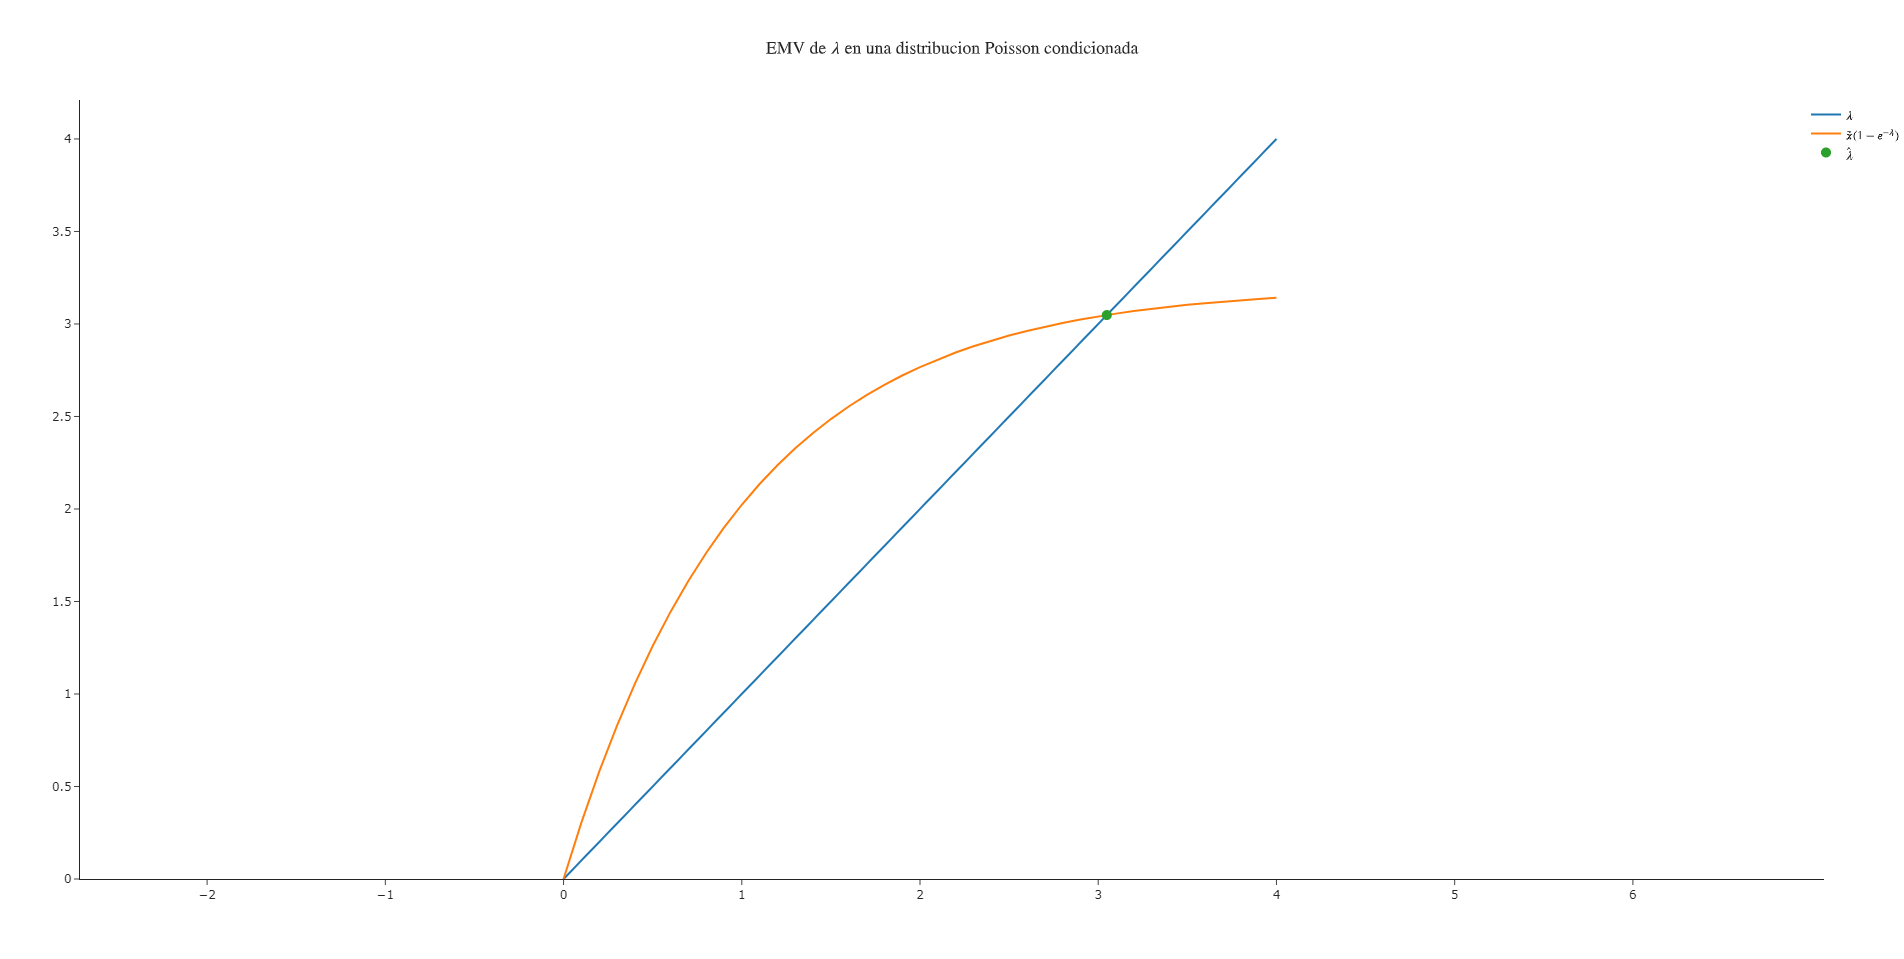
\includegraphics[scale=0.22]{Images/emv.png}
				\end{center}
			\end{figure}

			Se anexa código.
		\end{sol}
	\end{enumerate}
\end{document}

